% Options for packages loaded elsewhere
\PassOptionsToPackage{unicode}{hyperref}
\PassOptionsToPackage{hyphens}{url}
%
\documentclass[
  12pt,
]{article}
\title{Comparison of Avian Clutch Size, Physical Characterists, and
Mating Tactics}
\usepackage{etoolbox}
\makeatletter
\providecommand{\subtitle}[1]{% add subtitle to \maketitle
  \apptocmd{\@title}{\par {\large #1 \par}}{}{}
}
\makeatother
\subtitle{\url{https://github.com/jcf55/Fahrenholz_Costes_ENV872_EDA_FinalProject}}
\author{Lydie Costes and Jackie Fahrenholz}
\date{}

\usepackage{amsmath,amssymb}
\usepackage{lmodern}
\usepackage{iftex}
\ifPDFTeX
  \usepackage[T1]{fontenc}
  \usepackage[utf8]{inputenc}
  \usepackage{textcomp} % provide euro and other symbols
\else % if luatex or xetex
  \usepackage{unicode-math}
  \defaultfontfeatures{Scale=MatchLowercase}
  \defaultfontfeatures[\rmfamily]{Ligatures=TeX,Scale=1}
  \setmainfont[]{Times New Roman}
\fi
% Use upquote if available, for straight quotes in verbatim environments
\IfFileExists{upquote.sty}{\usepackage{upquote}}{}
\IfFileExists{microtype.sty}{% use microtype if available
  \usepackage[]{microtype}
  \UseMicrotypeSet[protrusion]{basicmath} % disable protrusion for tt fonts
}{}
\makeatletter
\@ifundefined{KOMAClassName}{% if non-KOMA class
  \IfFileExists{parskip.sty}{%
    \usepackage{parskip}
  }{% else
    \setlength{\parindent}{0pt}
    \setlength{\parskip}{6pt plus 2pt minus 1pt}}
}{% if KOMA class
  \KOMAoptions{parskip=half}}
\makeatother
\usepackage{xcolor}
\IfFileExists{xurl.sty}{\usepackage{xurl}}{} % add URL line breaks if available
\IfFileExists{bookmark.sty}{\usepackage{bookmark}}{\usepackage{hyperref}}
\hypersetup{
  pdftitle={Comparison of Avian Clutch Size, Physical Characterists, and Mating Tactics},
  pdfauthor={Lydie Costes and Jackie Fahrenholz},
  hidelinks,
  pdfcreator={LaTeX via pandoc}}
\urlstyle{same} % disable monospaced font for URLs
\usepackage[margin=2.54cm]{geometry}
\usepackage{color}
\usepackage{fancyvrb}
\newcommand{\VerbBar}{|}
\newcommand{\VERB}{\Verb[commandchars=\\\{\}]}
\DefineVerbatimEnvironment{Highlighting}{Verbatim}{commandchars=\\\{\}}
% Add ',fontsize=\small' for more characters per line
\usepackage{framed}
\definecolor{shadecolor}{RGB}{248,248,248}
\newenvironment{Shaded}{\begin{snugshade}}{\end{snugshade}}
\newcommand{\AlertTok}[1]{\textcolor[rgb]{0.94,0.16,0.16}{#1}}
\newcommand{\AnnotationTok}[1]{\textcolor[rgb]{0.56,0.35,0.01}{\textbf{\textit{#1}}}}
\newcommand{\AttributeTok}[1]{\textcolor[rgb]{0.77,0.63,0.00}{#1}}
\newcommand{\BaseNTok}[1]{\textcolor[rgb]{0.00,0.00,0.81}{#1}}
\newcommand{\BuiltInTok}[1]{#1}
\newcommand{\CharTok}[1]{\textcolor[rgb]{0.31,0.60,0.02}{#1}}
\newcommand{\CommentTok}[1]{\textcolor[rgb]{0.56,0.35,0.01}{\textit{#1}}}
\newcommand{\CommentVarTok}[1]{\textcolor[rgb]{0.56,0.35,0.01}{\textbf{\textit{#1}}}}
\newcommand{\ConstantTok}[1]{\textcolor[rgb]{0.00,0.00,0.00}{#1}}
\newcommand{\ControlFlowTok}[1]{\textcolor[rgb]{0.13,0.29,0.53}{\textbf{#1}}}
\newcommand{\DataTypeTok}[1]{\textcolor[rgb]{0.13,0.29,0.53}{#1}}
\newcommand{\DecValTok}[1]{\textcolor[rgb]{0.00,0.00,0.81}{#1}}
\newcommand{\DocumentationTok}[1]{\textcolor[rgb]{0.56,0.35,0.01}{\textbf{\textit{#1}}}}
\newcommand{\ErrorTok}[1]{\textcolor[rgb]{0.64,0.00,0.00}{\textbf{#1}}}
\newcommand{\ExtensionTok}[1]{#1}
\newcommand{\FloatTok}[1]{\textcolor[rgb]{0.00,0.00,0.81}{#1}}
\newcommand{\FunctionTok}[1]{\textcolor[rgb]{0.00,0.00,0.00}{#1}}
\newcommand{\ImportTok}[1]{#1}
\newcommand{\InformationTok}[1]{\textcolor[rgb]{0.56,0.35,0.01}{\textbf{\textit{#1}}}}
\newcommand{\KeywordTok}[1]{\textcolor[rgb]{0.13,0.29,0.53}{\textbf{#1}}}
\newcommand{\NormalTok}[1]{#1}
\newcommand{\OperatorTok}[1]{\textcolor[rgb]{0.81,0.36,0.00}{\textbf{#1}}}
\newcommand{\OtherTok}[1]{\textcolor[rgb]{0.56,0.35,0.01}{#1}}
\newcommand{\PreprocessorTok}[1]{\textcolor[rgb]{0.56,0.35,0.01}{\textit{#1}}}
\newcommand{\RegionMarkerTok}[1]{#1}
\newcommand{\SpecialCharTok}[1]{\textcolor[rgb]{0.00,0.00,0.00}{#1}}
\newcommand{\SpecialStringTok}[1]{\textcolor[rgb]{0.31,0.60,0.02}{#1}}
\newcommand{\StringTok}[1]{\textcolor[rgb]{0.31,0.60,0.02}{#1}}
\newcommand{\VariableTok}[1]{\textcolor[rgb]{0.00,0.00,0.00}{#1}}
\newcommand{\VerbatimStringTok}[1]{\textcolor[rgb]{0.31,0.60,0.02}{#1}}
\newcommand{\WarningTok}[1]{\textcolor[rgb]{0.56,0.35,0.01}{\textbf{\textit{#1}}}}
\usepackage{longtable,booktabs,array}
\usepackage{calc} % for calculating minipage widths
% Correct order of tables after \paragraph or \subparagraph
\usepackage{etoolbox}
\makeatletter
\patchcmd\longtable{\par}{\if@noskipsec\mbox{}\fi\par}{}{}
\makeatother
% Allow footnotes in longtable head/foot
\IfFileExists{footnotehyper.sty}{\usepackage{footnotehyper}}{\usepackage{footnote}}
\makesavenoteenv{longtable}
\usepackage{graphicx}
\makeatletter
\def\maxwidth{\ifdim\Gin@nat@width>\linewidth\linewidth\else\Gin@nat@width\fi}
\def\maxheight{\ifdim\Gin@nat@height>\textheight\textheight\else\Gin@nat@height\fi}
\makeatother
% Scale images if necessary, so that they will not overflow the page
% margins by default, and it is still possible to overwrite the defaults
% using explicit options in \includegraphics[width, height, ...]{}
\setkeys{Gin}{width=\maxwidth,height=\maxheight,keepaspectratio}
% Set default figure placement to htbp
\makeatletter
\def\fps@figure{htbp}
\makeatother
\setlength{\emergencystretch}{3em} % prevent overfull lines
\providecommand{\tightlist}{%
  \setlength{\itemsep}{0pt}\setlength{\parskip}{0pt}}
\setcounter{secnumdepth}{5}
\ifLuaTeX
  \usepackage{selnolig}  % disable illegal ligatures
\fi

\begin{document}
\maketitle

\newpage
\tableofcontents 
\newpage
\listoftables 
\listoffigures 
\newpage

\hypertarget{rationale-and-research-questions}{%
\section{Rationale and Research
Questions}\label{rationale-and-research-questions}}

According to the study from which this data was extracted, avian body
size and the evolution of birds over time is a highly debated subject
matter. Generally, there is agreement around the idea that body size of
bird species impacts other characteristics. Because of this, this
project intends to explore the correlation between body size and various
measurements and observations in our data.

First, we ask the question if female tail size predicts clutch size.
Tail length has a significant impact on control and agility (Evans
1999). Longer tails increase crash risk as well as reduces the ability
to maneuver (Evans 1999). We believe that this may have an overall
negative impact on clutch size, as birds with longer tail lengths may be
less efficient at collecting food for their young. Second, we will
explore interactions between male tail length and methods of display,
mating system, and resource sharing systems. Tail length likely has a
negative impact on navigation, and collecting food, while having a
positive impact on sexual display. Physical characteristics of males are
evaluated by females in search of a mate.

\hypertarget{dataset-information}{%
\section{Dataset Information}\label{dataset-information}}

Our dataset consists of data that was collected starting in 2005 and was
last updated in January of 2007. Data for this collection come from
regions that include:

\begin{itemize}
\tightlist
\item
  Western Palearctic
\item
  Neararctic
\item
  Africa
\item
  Australia
\item
  New Zealand
\item
  Antarctica
\end{itemize}

The complete dataset (represented below by the variable \texttt{birds})
includes 41 variables, and represents 125 families. According to the
metadata, the majority of this information was gathered from
ornithological handbooks, with some data obtained from personal
communications with authors who published information on species bird
groups. More information on the sources used can be found at:
\url{https://esapubs.org/archive/ecol/E088/096/metadata.htm} (also in
/Data/Raw in the .tex file)

\newpage

\hypertarget{exploratory-analysis}{%
\section{Exploratory Analysis}\label{exploratory-analysis}}

\begin{Shaded}
\begin{Highlighting}[]
\CommentTok{\#dimensions}
\FunctionTok{dim}\NormalTok{(birds)}
\end{Highlighting}
\end{Shaded}

\begin{verbatim}
## [1] 3769   41
\end{verbatim}

\begin{Shaded}
\begin{Highlighting}[]
\CommentTok{\#column names}
\FunctionTok{colnames}\NormalTok{(birds)}
\end{Highlighting}
\end{Shaded}

\begin{verbatim}
##  [1] "ï..Family"        "Species_number"   "Species_name"     "English_name"    
##  [5] "Subspecies"       "M_mass"           "M_mass_N"         "F_mass"          
##  [9] "F_mass_N"         "unsexed_mass"     "unsexed_mass_N"   "M_wing"          
## [13] "M_wing_N"         "F_wing"           "F_wing_N"         "Unsexed_wing"    
## [17] "Unsexed_wing_N"   "M_tarsus"         "M_tarsus_N"       "F_tarsus"        
## [21] "F_tarsus_N"       "Unsexed_tarsus"   "Unsexed_tarsus_N" "M_bill"          
## [25] "M_bill_N"         "F_bill"           "F_bill_N"         "Unsexed_bill"    
## [29] "Unsexed_bill_N"   "M_tail"           "M_tail_N"         "F_tail"          
## [33] "F_tail_N"         "Unsexed_tail"     "Unsexed_tail_N"   "Clutch_size"     
## [37] "Egg_mass"         "Mating_System"    "Display"          "Resource"        
## [41] "References"
\end{verbatim}

\begin{Shaded}
\begin{Highlighting}[]
\CommentTok{\#variable types?}
\FunctionTok{str}\NormalTok{(birds)}
\end{Highlighting}
\end{Shaded}

\begin{verbatim}
## 'data.frame':    3769 obs. of  41 variables:
##  $ ï..Family       : int  115 101 116 116 116 116 116 116 116 116 ...
##  $ Species_number  : int  5351 3964 5402 5398 5400 5401 5396 5405 5404 5397 ...
##  $ Species_name    : chr  "Acanthagenys rufogularis" "Acanthisitta chloris" "Acanthiza chrysorrhoa" "Acanthiza ewingii" ...
##  $ English_name    : chr  "Spiny-cheeked Honeyeater" "Rifleman" "Yellow-rumped Thornbill" "Tasmanian Thornbill" ...
##  $ Subspecies      : chr  "-999" "-999" "leighi" "ewingii" ...
##  $ M_mass          : num  47.1 5.6 9.4 7.2 7.2 5.8 6.8 7.6 6.5 7.4 ...
##  $ M_mass_N        : int  4 33 25 16 43 16 10 25 27 37 ...
##  $ F_mass          : num  41.4 7 9.8 6.7 6.9 5.7 6.7 7.4 6.3 6.5 ...
##  $ F_mass_N        : int  5 20 16 19 76 12 7 27 23 20 ...
##  $ unsexed_mass    : num  -999 -999 -999 -999 -999 -999 -999 -999 -999 -999 ...
##  $ unsexed_mass_N  : int  -999 -999 -999 -999 -999 -999 -999 -999 -999 -999 ...
##  $ M_wing          : num  113.1 47.8 57.8 52.7 48.9 ...
##  $ M_wing_N        : int  25 10 25 21 28 29 11 36 25 52 ...
##  $ F_wing          : num  107.5 51.4 57.6 51 47 ...
##  $ F_wing_N        : num  21 10 26 22 26 25 7 26 29 30 ...
##  $ Unsexed_wing    : num  -999 -999 -999 -999 -999 -999 -999 -999 -999 -999 ...
##  $ Unsexed_wing_N  : int  -999 -999 -999 -999 -999 -999 -999 -999 -999 -999 ...
##  $ M_tarsus        : num  26.2 19.1 17.7 21.3 18 18.4 18.5 17.5 17.4 20.3 ...
##  $ M_tarsus_N      : int  10 10 23 21 28 29 11 36 25 51 ...
##  $ F_tarsus        : num  25.7 19.7 17.4 21.7 17.8 17.6 18.4 17.5 17.3 19.3 ...
##  $ F_tarsus_N      : int  5 7 24 23 25 25 7 25 27 29 ...
##  $ Unsexed_tarsus  : num  -999 -999 -999 -999 -999 -999 -999 -999 -999 -999 ...
##  $ Unsexed_tarsus_N: int  -999 -999 -999 -999 -999 -999 -999 -999 -999 -999 ...
##  $ M_bill          : num  26.8 13.2 11.9 11 11.3 9.7 11.6 10.2 10 11 ...
##  $ M_bill_N        : int  8 6 24 21 27 28 11 26 24 51 ...
##  $ F_bill          : num  25.5 14.4 11.7 10.9 11.4 9.6 11.2 9.9 10 10.5 ...
##  $ F_bill_N        : num  10 7 26 23 25 24 7 26 28 29 ...
##  $ Unsexed_bill    : num  -999 -999 -999 -999 -999 -999 -999 -999 -999 -999 ...
##  $ Unsexed_bill_N  : int  -999 -999 -999 -999 -999 -999 -999 -999 -999 -999 ...
##  $ M_tail          : num  113.4 23.3 40.8 47.8 36.3 ...
##  $ M_tail_N        : int  25 10 28 21 34 28 11 36 14 51 ...
##  $ F_tail          : num  106.4 22.1 39.3 46.8 35.4 ...
##  $ F_tail_N        : int  21 7 26 23 55 25 6 26 10 30 ...
##  $ Unsexed_tail    : num  -999 -999 -999 -999 -999 -999 -999 -999 -999 -999 ...
##  $ Unsexed_tail_N  : int  -999 -999 -999 -999 -999 -999 -999 -999 -999 -999 ...
##  $ Clutch_size     : num  2.2 4 3.5 3.5 3 3 2.5 3 3 3 ...
##  $ Egg_mass        : num  5.45 1.34 1.44 1.46 1.35 0.93 -999 1.32 1.34 1.4 ...
##  $ Mating_System   : int  2 2 2 2 2 -999 -999 2 2 2 ...
##  $ Display         : int  3 1 1 1 -999 1 -999 2 -999 1 ...
##  $ Resource        : int  2 2 1 0 1 1 -999 0 -999 2 ...
##  $ References      : chr  "1, 21" "21" "1, 22, 31 " "22, 31" ...
\end{verbatim}

\begin{Shaded}
\begin{Highlighting}[]
\CommentTok{\#look at the first few lines}
\FunctionTok{head}\NormalTok{(birds)}
\end{Highlighting}
\end{Shaded}

\begin{verbatim}
##   ï..Family Species_number             Species_name             English_name
## 1       115           5351 Acanthagenys rufogularis Spiny-cheeked Honeyeater
## 2       101           3964     Acanthisitta chloris                 Rifleman
## 3       116           5402    Acanthiza chrysorrhoa  Yellow-rumped Thornbill
## 4       116           5398        Acanthiza ewingii      Tasmanian Thornbill
## 5       116           5400       Acanthiza inornata        Western Thornbill
## 6       116           5401       Acanthiza iredalei Slender-billed Thornbill
##   Subspecies M_mass M_mass_N F_mass F_mass_N unsexed_mass unsexed_mass_N M_wing
## 1       -999   47.1        4   41.4        5         -999           -999  113.1
## 2       -999    5.6       33    7.0       20         -999           -999   47.8
## 3     leighi    9.4       25    9.8       16         -999           -999   57.8
## 4    ewingii    7.2       16    6.7       19         -999           -999   52.7
## 5       -999    7.2       43    6.9       76         -999           -999   48.9
## 6   iredalei    5.8       16    5.7       12         -999           -999   48.8
##   M_wing_N F_wing F_wing_N Unsexed_wing Unsexed_wing_N M_tarsus M_tarsus_N
## 1       25  107.5       21         -999           -999     26.2         10
## 2       10   51.4       10         -999           -999     19.1         10
## 3       25   57.6       26         -999           -999     17.7         23
## 4       21   51.0       22         -999           -999     21.3         21
## 5       28   47.0       26         -999           -999     18.0         28
## 6       29   47.5       25         -999           -999     18.4         29
##   F_tarsus F_tarsus_N Unsexed_tarsus Unsexed_tarsus_N M_bill M_bill_N F_bill
## 1     25.7          5           -999             -999   26.8        8   25.5
## 2     19.7          7           -999             -999   13.2        6   14.4
## 3     17.4         24           -999             -999   11.9       24   11.7
## 4     21.7         23           -999             -999   11.0       21   10.9
## 5     17.8         25           -999             -999   11.3       27   11.4
## 6     17.6         25           -999             -999    9.7       28    9.6
##   F_bill_N Unsexed_bill Unsexed_bill_N M_tail M_tail_N F_tail F_tail_N
## 1       10         -999           -999  113.4       25  106.4       21
## 2        7         -999           -999   23.3       10   22.1        7
## 3       26         -999           -999   40.8       28   39.3       26
## 4       23         -999           -999   47.8       21   46.8       23
## 5       25         -999           -999   36.3       34   35.4       55
## 6       24         -999           -999   40.6       28   39.6       25
##   Unsexed_tail Unsexed_tail_N Clutch_size Egg_mass Mating_System Display
## 1         -999           -999         2.2     5.45             2       3
## 2         -999           -999         4.0     1.34             2       1
## 3         -999           -999         3.5     1.44             2       1
## 4         -999           -999         3.5     1.46             2       1
## 5         -999           -999         3.0     1.35             2    -999
## 6         -999           -999         3.0     0.93          -999       1
##   Resource References
## 1        2      1, 21
## 2        2         21
## 3        1 1, 22, 31 
## 4        0     22, 31
## 5        1     22, 31
## 6        1     22, 31
\end{verbatim}

\begin{Shaded}
\begin{Highlighting}[]
\CommentTok{\# make sure family column is named correctly}
\FunctionTok{colnames}\NormalTok{(birds)[}\DecValTok{1}\NormalTok{] }\OtherTok{\textless{}{-}} \StringTok{"Family"}
\end{Highlighting}
\end{Shaded}

\begin{Shaded}
\begin{Highlighting}[]
\CommentTok{\# Convert {-}999 to NAs and add genus column}
\NormalTok{birds }\OtherTok{\textless{}{-}}\NormalTok{ birds }\SpecialCharTok{\%\textgreater{}\%}
  \FunctionTok{na\_if}\NormalTok{(., }\SpecialCharTok{{-}}\DecValTok{999}\NormalTok{) }\SpecialCharTok{\%\textgreater{}\%}
  \FunctionTok{separate}\NormalTok{(Species\_name, }
           \AttributeTok{sep =} \StringTok{" "}\NormalTok{, }
           \AttributeTok{into =} \FunctionTok{c}\NormalTok{(}\StringTok{"Genus"}\NormalTok{, }\StringTok{"Sp"}\NormalTok{), }
           \AttributeTok{remove =} \ConstantTok{FALSE}\NormalTok{)}

\CommentTok{\# Subset to columns we are interested in}
\NormalTok{birds.subset }\OtherTok{\textless{}{-}}\NormalTok{ birds }\SpecialCharTok{\%\textgreater{}\%}
  \FunctionTok{select}\NormalTok{(Family, Species\_name, Genus, F\_mass, M\_mass, }
\NormalTok{         F\_tail, M\_tail, Clutch\_size, Mating\_System, }
\NormalTok{         Display, Resource)}

\CommentTok{\# This function allows calculation of mode for categorical variables}
\NormalTok{Mode }\OtherTok{\textless{}{-}} \ControlFlowTok{function}\NormalTok{(x) \{}
\NormalTok{  ux }\OtherTok{\textless{}{-}} \FunctionTok{unique}\NormalTok{(x) }
\NormalTok{  ux[}\FunctionTok{which.max}\NormalTok{(}\FunctionTok{tabulate}\NormalTok{(}\FunctionTok{match}\NormalTok{(x, ux)))]}
\NormalTok{\}}

\CommentTok{\# Group male tail length by mating system to graph later}
\NormalTok{birds.mating.tail }\OtherTok{\textless{}{-}}\NormalTok{ birds.subset }\SpecialCharTok{\%\textgreater{}\%}
  \FunctionTok{group\_by}\NormalTok{(Mating\_System) }\SpecialCharTok{\%\textgreater{}\%}
  \FunctionTok{summarise}\NormalTok{(}\AttributeTok{M\_tail =} \FunctionTok{mean}\NormalTok{(M\_tail, }\AttributeTok{na.rm =} \ConstantTok{TRUE}\NormalTok{))}

\CommentTok{\# Group by family, average by mean or mode}
\NormalTok{birds.family }\OtherTok{\textless{}{-}}\NormalTok{ birds.subset }\SpecialCharTok{\%\textgreater{}\%}
  \FunctionTok{group\_by}\NormalTok{(Family) }\SpecialCharTok{\%\textgreater{}\%} 
  \FunctionTok{summarise}\NormalTok{(}\AttributeTok{F\_mass =} \FunctionTok{mean}\NormalTok{(F\_mass, }\AttributeTok{na.rm =} \ConstantTok{TRUE}\NormalTok{),}
            \AttributeTok{M\_mass =} \FunctionTok{mean}\NormalTok{(M\_mass, }\AttributeTok{na.rm =} \ConstantTok{TRUE}\NormalTok{),}
            \AttributeTok{F\_tail =} \FunctionTok{mean}\NormalTok{(F\_tail, }\AttributeTok{na.rm =} \ConstantTok{TRUE}\NormalTok{),}
            \AttributeTok{M\_tail =} \FunctionTok{mean}\NormalTok{(M\_tail, }\AttributeTok{na.rm =} \ConstantTok{TRUE}\NormalTok{),}
            \AttributeTok{Clutch\_size =} \FunctionTok{mean}\NormalTok{(Clutch\_size, }\AttributeTok{na.rm =} \ConstantTok{TRUE}\NormalTok{),}
            \AttributeTok{Common\_Mating\_System =} \FunctionTok{Mode}\NormalTok{(Mating\_System),}
            \AttributeTok{Common\_Display =} \FunctionTok{Mode}\NormalTok{(Display),}
            \AttributeTok{Common\_Resource =} \FunctionTok{Mode}\NormalTok{(Resource)) }\SpecialCharTok{\%\textgreater{}\%}
  \FunctionTok{filter}\NormalTok{(}\SpecialCharTok{!}\FunctionTok{is.na}\NormalTok{(Clutch\_size), }\SpecialCharTok{!}\FunctionTok{is.na}\NormalTok{(F\_tail), }
         \SpecialCharTok{!}\FunctionTok{is.na}\NormalTok{(F\_mass), }\SpecialCharTok{!}\FunctionTok{is.na}\NormalTok{(M\_tail))}

\CommentTok{\# Set categorical variables as factors}
\NormalTok{birds.subset}\SpecialCharTok{$}\NormalTok{Family }\OtherTok{\textless{}{-}} \FunctionTok{as.factor}\NormalTok{(birds.subset}\SpecialCharTok{$}\NormalTok{Family)}
\NormalTok{birds.subset}\SpecialCharTok{$}\NormalTok{Mating\_System }\OtherTok{\textless{}{-}} \FunctionTok{as.factor}\NormalTok{(birds.subset}\SpecialCharTok{$}\NormalTok{Mating\_System)}
\NormalTok{birds.subset}\SpecialCharTok{$}\NormalTok{Display }\OtherTok{\textless{}{-}} \FunctionTok{as.factor}\NormalTok{(birds.subset}\SpecialCharTok{$}\NormalTok{Display)}
\NormalTok{birds.subset}\SpecialCharTok{$}\NormalTok{Resource }\OtherTok{\textless{}{-}} \FunctionTok{as.factor}\NormalTok{(birds.subset}\SpecialCharTok{$}\NormalTok{Resource)}

\CommentTok{\# Write the csv file into our Processed data folder}
\FunctionTok{write.csv}\NormalTok{(birds.subset, }\AttributeTok{file =} \StringTok{"../Data/Processed/birds\_subset.csv"}\NormalTok{)}
\FunctionTok{write.csv}\NormalTok{(birds.family, }\AttributeTok{file =} \StringTok{"../Data/Processed/birds\_family.csv"}\NormalTok{)}
\end{Highlighting}
\end{Shaded}

\begin{Shaded}
\begin{Highlighting}[]
\CommentTok{\# View variable distributions and relationships}
\NormalTok{gg.birds.subset }\OtherTok{\textless{}{-}} \FunctionTok{subset}\NormalTok{(birds.subset, }\AttributeTok{select =} \SpecialCharTok{{-}}\FunctionTok{c}\NormalTok{(Family, Species\_name, Genus))}
\FunctionTok{ggpairs}\NormalTok{(gg.birds.subset)}
\end{Highlighting}
\end{Shaded}

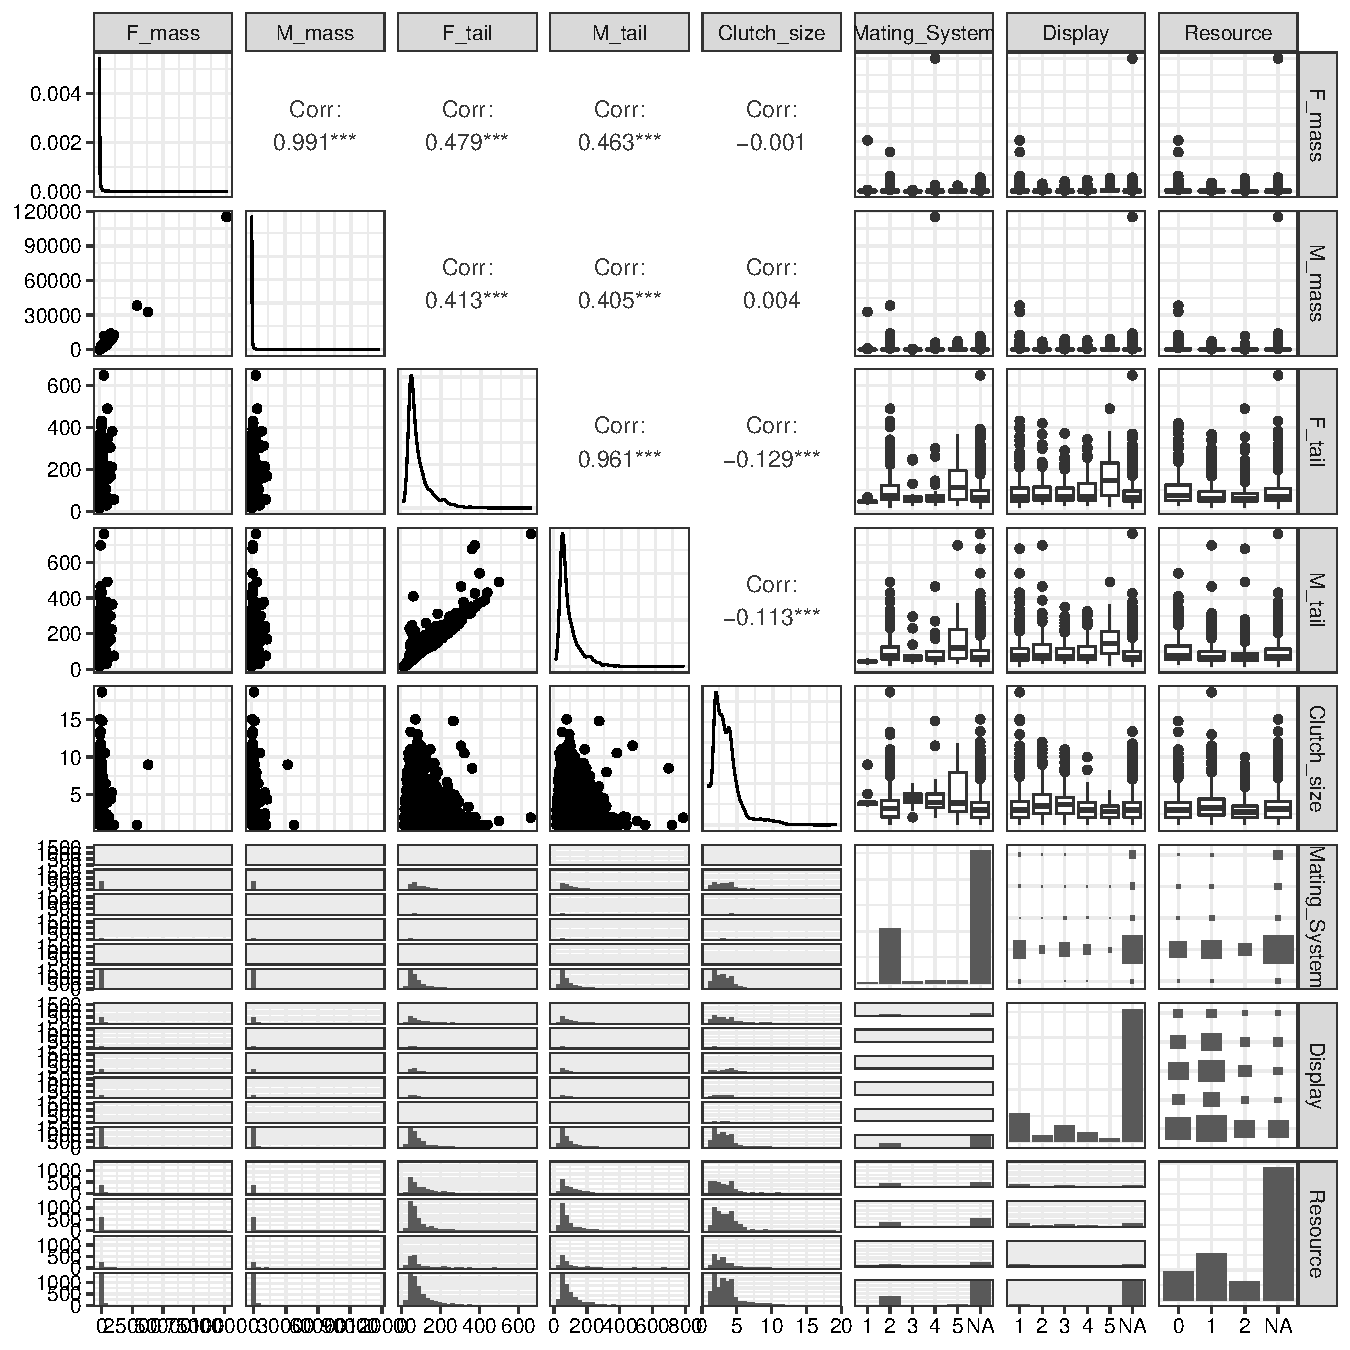
\includegraphics{Project_Code_files/figure-latex/gg exploration-1.pdf}

\begin{Shaded}
\begin{Highlighting}[]
\CommentTok{\# View the counts of our factor variables}
\FunctionTok{count}\NormalTok{(birds.subset, }\AttributeTok{vars =}\NormalTok{ Mating\_System) }
\end{Highlighting}
\end{Shaded}

\begin{verbatim}
##   vars    n
## 1    1   23
## 2    2 1057
## 3    3   36
## 4    4   46
## 5    5   56
## 6 <NA> 2551
\end{verbatim}

\begin{Shaded}
\begin{Highlighting}[]
\CommentTok{\# SUPER uneven! This could be an issue contributing to uneven variances?}
\FunctionTok{count}\NormalTok{(birds.subset, }\AttributeTok{vars =}\NormalTok{ Display) }\CommentTok{\# Also uneven but not quite as bad}
\end{Highlighting}
\end{Shaded}

\begin{verbatim}
##   vars    n
## 1    1  549
## 2    2  118
## 3    3  311
## 4    4  186
## 5    5   54
## 6 <NA> 2551
\end{verbatim}

\begin{Shaded}
\begin{Highlighting}[]
\FunctionTok{count}\NormalTok{(birds.subset, }\AttributeTok{vars =}\NormalTok{ Resource) }\CommentTok{\# Looks fine}
\end{Highlighting}
\end{Shaded}

\begin{verbatim}
##   vars    n
## 1    0  480
## 2    1  780
## 3    2  314
## 4 <NA> 2195
\end{verbatim}

\begin{longtable}[]{@{}lrrrrrrrr@{}}
\caption{Summary Statistics for Continuous Variables}\tabularnewline
\toprule
& vars & n & mean & sd & min & max & range & se \\
\midrule
\endfirsthead
\toprule
& vars & n & mean & sd & min & max & range & se \\
\midrule
\endhead
F\_mass & 1 & 2706 & 411.472616 & 2320.49997 & 1.8 & 100000.0 & 99998.2
& 44.6085053 \\
M\_mass & 2 & 2822 & 436.692275 & 2585.46747 & 2.0 & 115000.0 & 114998.0
& 48.6699134 \\
F\_tail & 3 & 2352 & 88.340901 & 59.91081 & 15.4 & 647.5 & 632.1 &
1.2353402 \\
M\_tail & 4 & 2390 & 92.410126 & 64.27592 & 15.8 & 762.0 & 746.2 &
1.3147688 \\
Clutch\_size & 5 & 2392 & 3.448037 & 1.88880 & 1.0 & 18.6 & 17.6 &
0.0386194 \\
\bottomrule
\end{longtable}

\begin{figure}
\centering
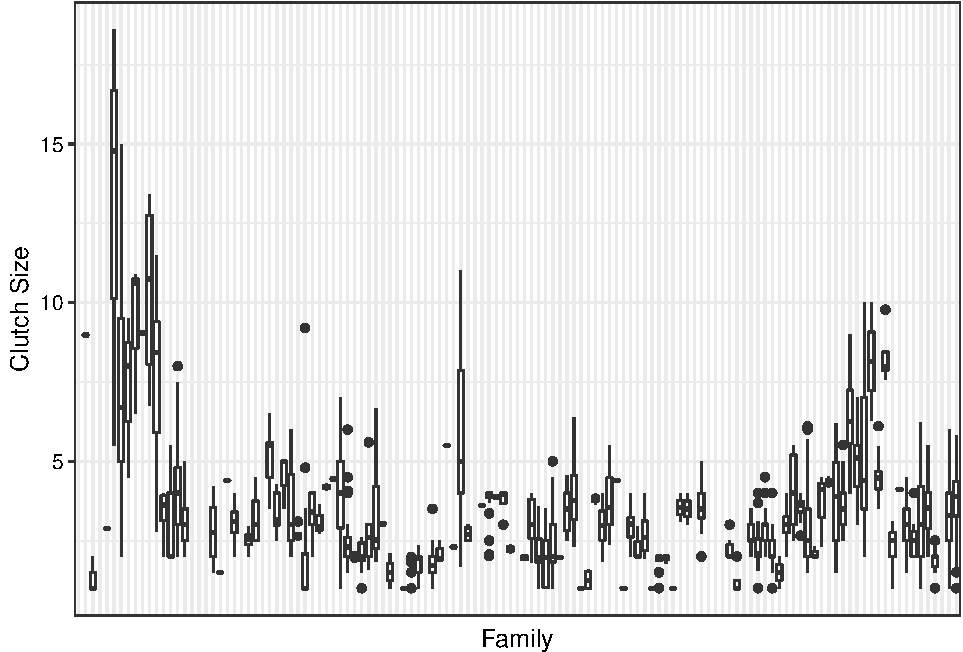
\includegraphics{Project_Code_files/figure-latex/exploratory_plots-1.pdf}
\caption{Exploratory Plot of Wrangled Data}
\end{figure}

\begin{figure}
\centering
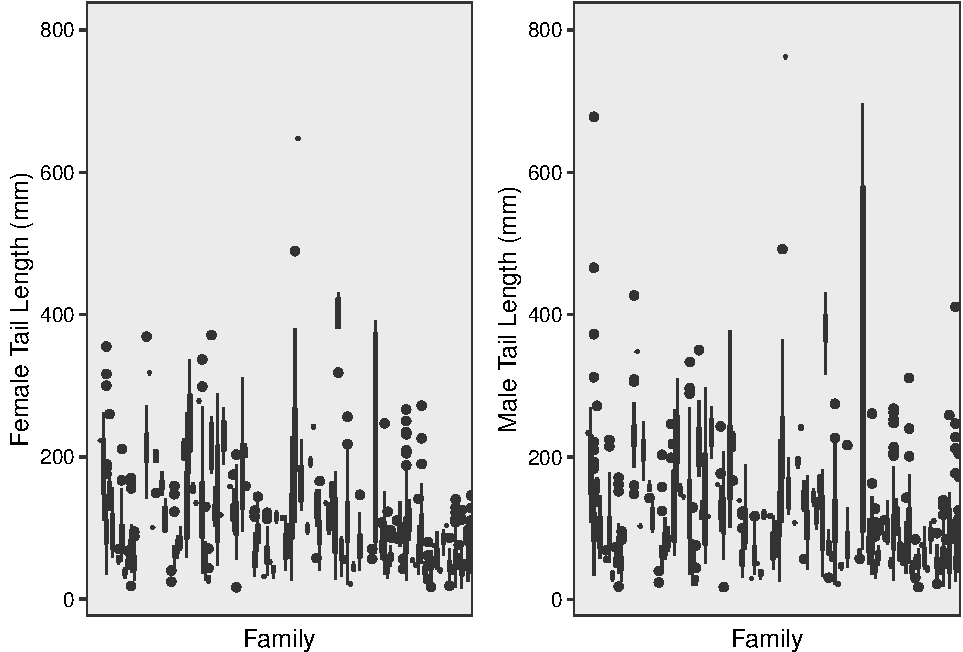
\includegraphics{Project_Code_files/figure-latex/r exploratory_plots_1-1.pdf}
\caption{Exploratory Plot of Wrangled Data}
\end{figure}

\begin{figure}
\centering
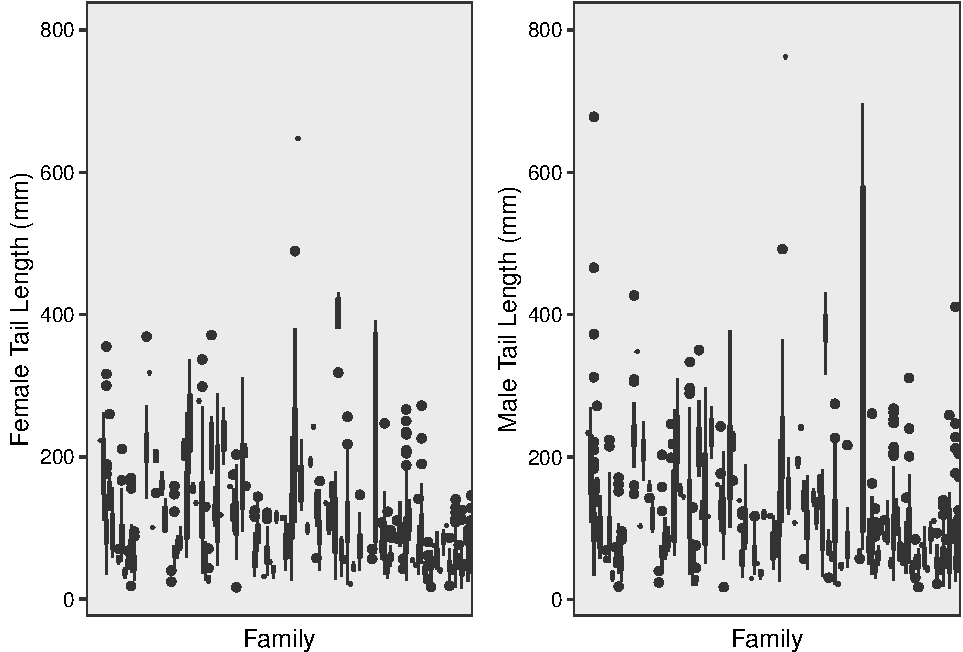
\includegraphics{Project_Code_files/figure-latex/r exploratory_plots_2-1.pdf}
\caption{Exploratory Plot of Wrangled Data}
\end{figure}

\begin{Shaded}
\begin{Highlighting}[]
\CommentTok{\# Run regression to compare male and female tail length}
\NormalTok{lm.tail }\OtherTok{\textless{}{-}} \FunctionTok{lm}\NormalTok{(}\AttributeTok{data =}\NormalTok{ birds.subset, M\_tail }\SpecialCharTok{\textasciitilde{}}\NormalTok{ F\_tail)}
\CommentTok{\# Check summary}
\FunctionTok{summary}\NormalTok{(lm.tail) }\CommentTok{\# highly correlated}
\end{Highlighting}
\end{Shaded}

\begin{verbatim}
## 
## Call:
## lm(formula = M_tail ~ F_tail, data = birds.subset)
## 
## Residuals:
##    Min     1Q Median     3Q    Max 
## -46.84  -3.21  -1.27   0.85 345.40 
## 
## Coefficients:
##             Estimate Std. Error t value Pr(>|t|)    
## (Intercept) 1.226565   0.652716   1.879   0.0603 .  
## F_tail      1.033250   0.006115 168.974   <2e-16 ***
## ---
## Signif. codes:  0 '***' 0.001 '**' 0.01 '*' 0.05 '.' 0.1 ' ' 1
## 
## Residual standard error: 17.76 on 2348 degrees of freedom
##   (1419 observations deleted due to missingness)
## Multiple R-squared:  0.924,  Adjusted R-squared:  0.924 
## F-statistic: 2.855e+04 on 1 and 2348 DF,  p-value: < 2.2e-16
\end{verbatim}

\begin{verbatim}
## `geom_smooth()` using formula 'y ~ x'
\end{verbatim}

\begin{figure}
\centering
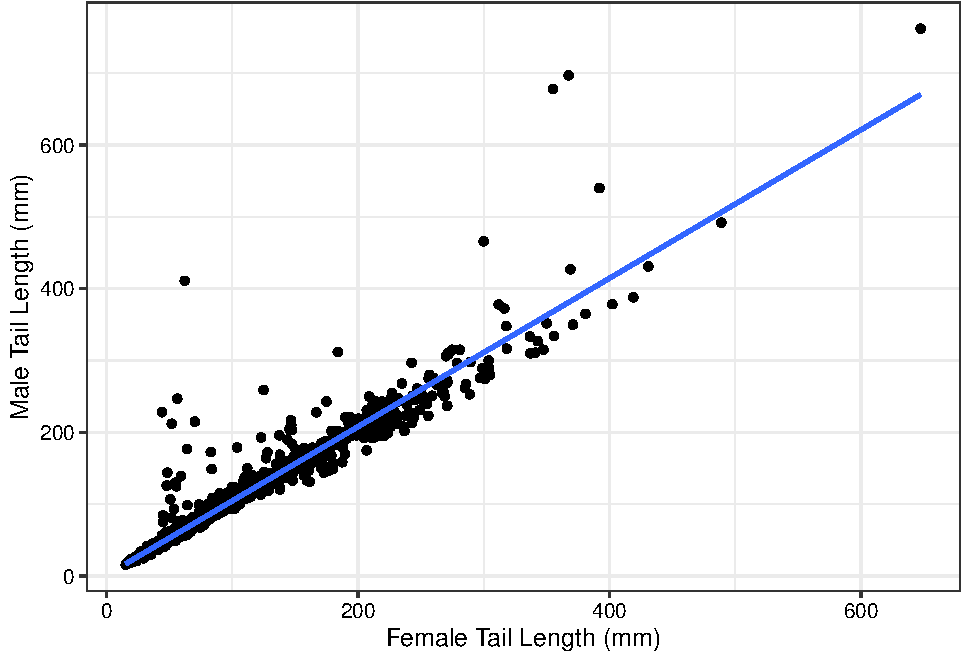
\includegraphics{Project_Code_files/figure-latex/r exploratory_plots_3-1.pdf}
\caption{Exploratory Plot of Wrangled Data}
\end{figure}

\begin{figure}
\centering
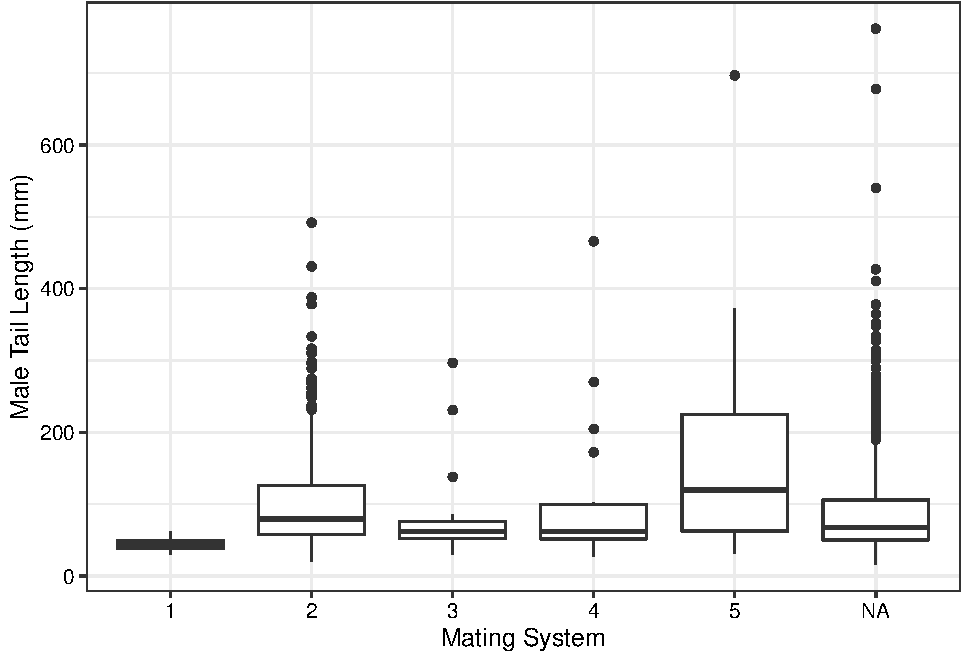
\includegraphics{Project_Code_files/figure-latex/r exploratory_plots_4-1.pdf}
\caption{Exploratory Plot of Wrangled Data}
\end{figure}

\begin{figure}
\centering
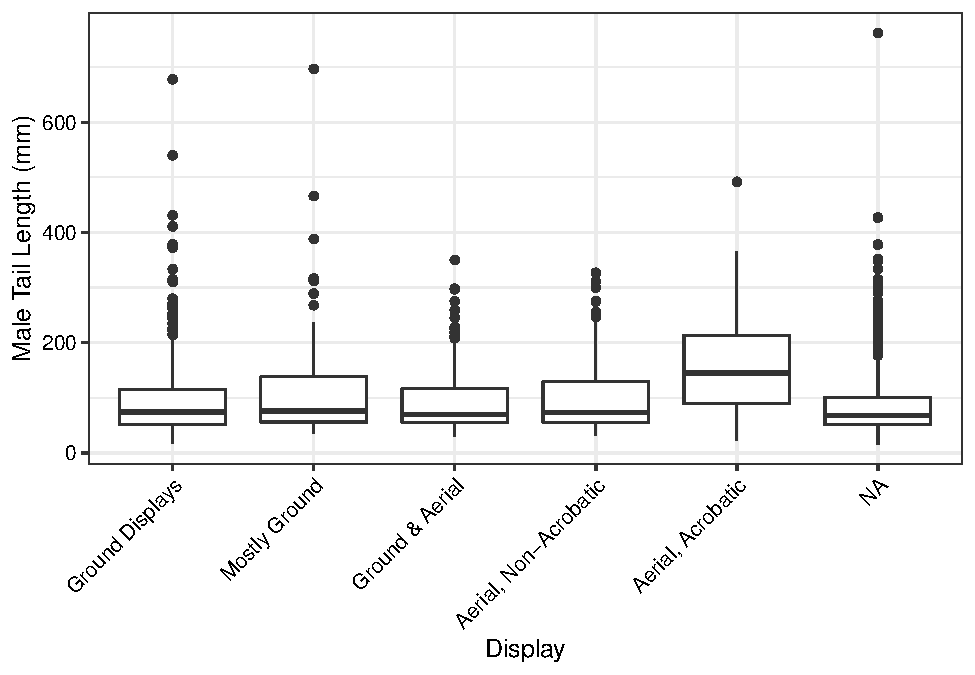
\includegraphics{Project_Code_files/figure-latex/r exploratory_plots_5-1.pdf}
\caption{Exploratory Plot of Wrangled Data}
\end{figure}

\begin{verbatim}
## Warning: Removed 1379 rows containing non-finite values (stat_boxplot).
\end{verbatim}

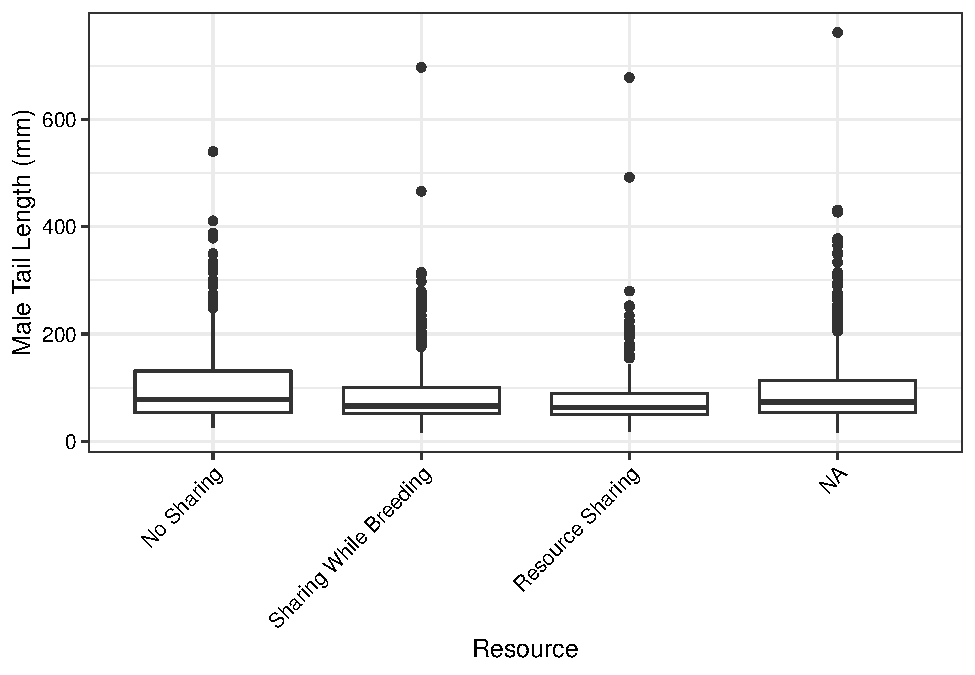
\includegraphics{Project_Code_files/figure-latex/exploratory_plots_6-1.pdf}
\newpage

\hypertarget{analysis}{%
\section{Analysis}\label{analysis}}

To test our hypotheses using our subset data \texttt{birds.subset}, we
will conduct a linear regression and an analysis of variance (ANOVA).
Our first research question will be answered using a linear regression,
while our second will be addressed with an ANOVA. Results will be
clearly stated in words, and supplemented using graphing visualizations.

\hypertarget{question-1-does-female-tail-length-predict-clutch-size}{%
\subsection{Question 1: Does female tail length predict clutch
size?}\label{question-1-does-female-tail-length-predict-clutch-size}}

\(H_0\) : There is no significant difference between female tail length
and clutch size.

\(H_A\) : There is a significant difference between female tail length
and clutch size.

Prior to conducting this anlaysis, it was identified that there is a
strong correlation between mass and tail length. We therefore included
this variable in our model, to see the further implications of this.

\begin{verbatim}
## 
## Call:
## lm(formula = F_mass ~ F_tail)
## 
## Residuals:
##     Min      1Q  Median      3Q     Max 
## -2100.1  -229.3   -65.0    36.4 11412.3 
## 
## Coefficients:
##             Estimate Std. Error t value Pr(>|t|)    
## (Intercept) -322.771     34.310  -9.407   <2e-16 ***
## F_tail         7.330      0.314  23.342   <2e-16 ***
## ---
## Signif. codes:  0 '***' 0.001 '**' 0.01 '*' 0.05 '.' 0.1 ' ' 1
## 
## Residual standard error: 826.3 on 1827 degrees of freedom
##   (1940 observations deleted due to missingness)
## Multiple R-squared:  0.2297, Adjusted R-squared:  0.2293 
## F-statistic: 544.9 on 1 and 1827 DF,  p-value: < 2.2e-16
\end{verbatim}

\begin{verbatim}
## 
## Call:
## lm(formula = Clutch_size ~ F_tail * F_mass)
## 
## Residuals:
##     Min      1Q  Median      3Q     Max 
## -4.9660 -1.2529 -0.2852  0.7347 11.9351 
## 
## Coefficients:
##                    Estimate    Std. Error t value  Pr(>|t|)    
## (Intercept)    3.8970630035  0.0920673618  42.328   < 2e-16 ***
## F_tail        -0.0038295564  0.0009331300  -4.104 0.0000426 ***
## F_mass         0.0002587737  0.0000979394   2.642   0.00832 ** 
## F_tail:F_mass -0.0000010753  0.0000004436  -2.424   0.01546 *  
## ---
## Signif. codes:  0 '***' 0.001 '**' 0.01 '*' 0.05 '.' 0.1 ' ' 1
## 
## Residual standard error: 1.891 on 1642 degrees of freedom
##   (2123 observations deleted due to missingness)
## Multiple R-squared:  0.02398,    Adjusted R-squared:  0.02219 
## F-statistic: 13.45 on 3 and 1642 DF,  p-value: 0.00000001141
\end{verbatim}

\begin{verbatim}
##        F_tail        F_mass F_tail:F_mass 
##      1.564475      4.086442      4.876822
\end{verbatim}

\begin{figure}
\centering
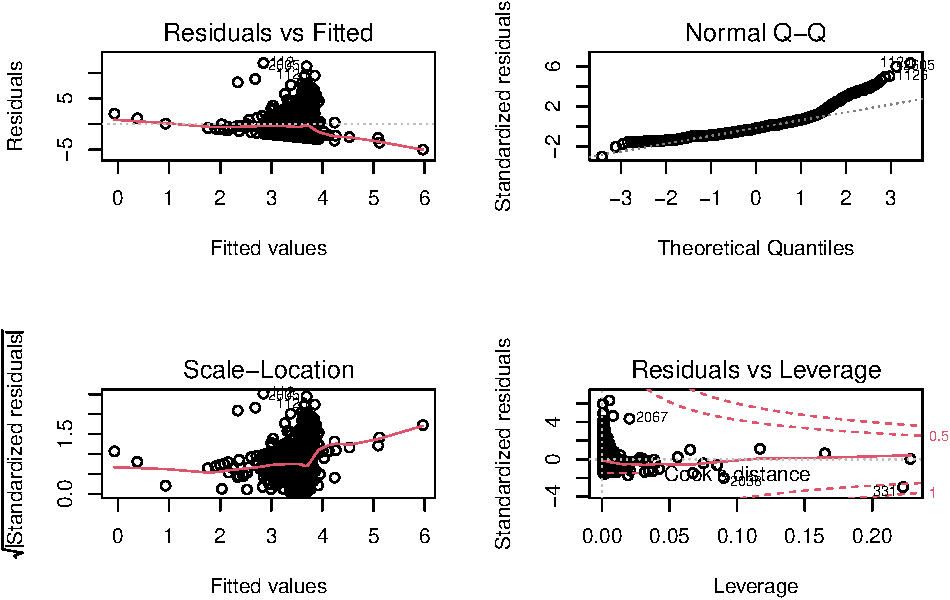
\includegraphics{Project_Code_files/figure-latex/q -1 residuals-1.pdf}
\caption{Residual Plots for Question 1}
\end{figure}

\begin{verbatim}
## `geom_smooth()` using formula 'y ~ x'
\end{verbatim}

\begin{figure}
\centering
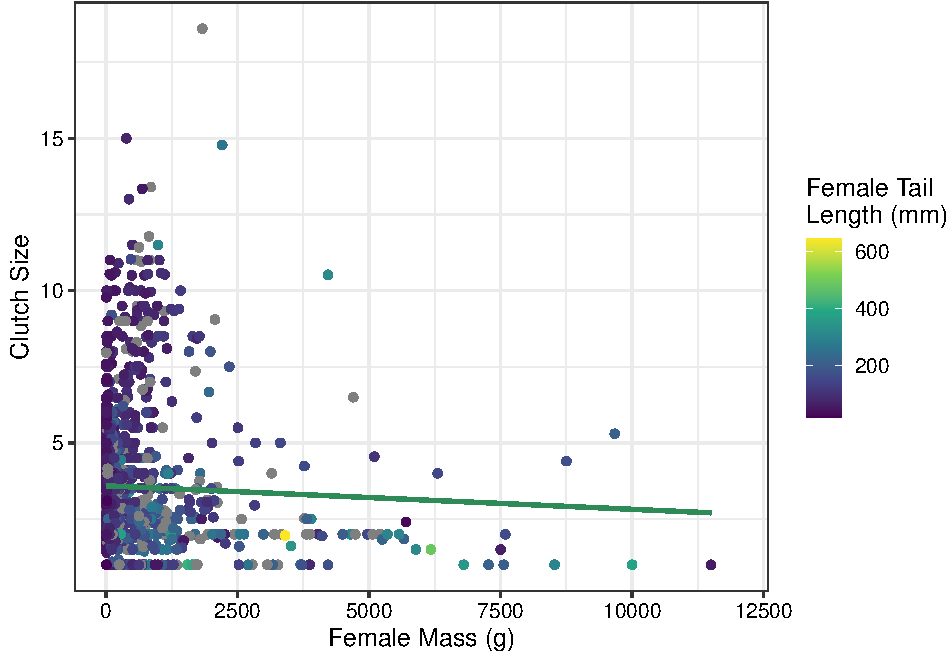
\includegraphics{Project_Code_files/figure-latex/q-1 plots-1.pdf}
\caption{Female Mass vs Clutch Size}
\end{figure}

\begin{verbatim}
## `geom_smooth()` using formula 'y ~ x'
\end{verbatim}

\begin{figure}
\centering
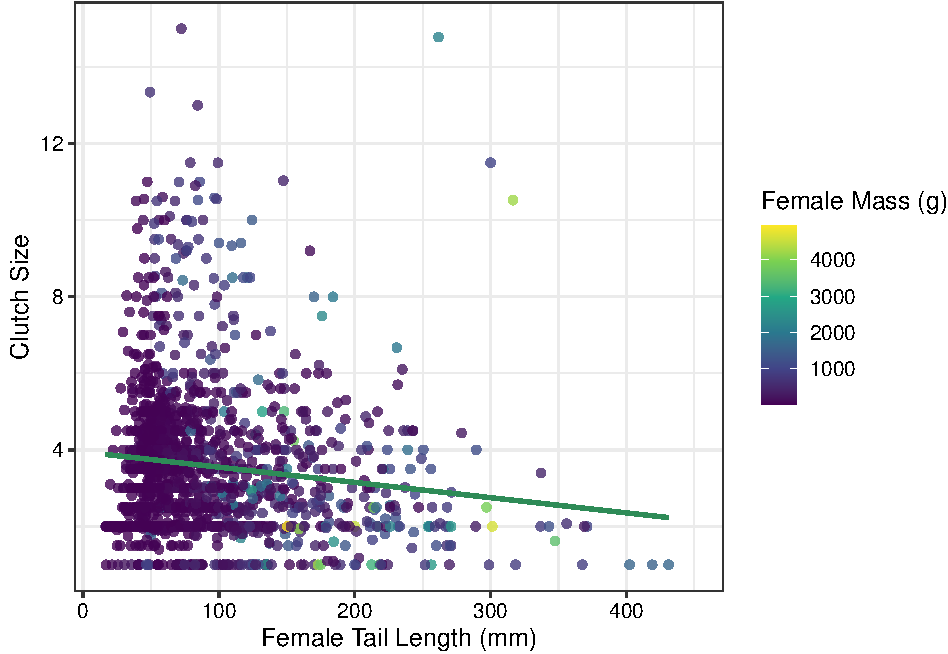
\includegraphics{Project_Code_files/figure-latex/q-1 plot zoom-1.pdf}
\caption{A Closer Look: Female Mass vs Clutch Size}
\end{figure}

\newpage

\hypertarget{question-2-does-male-tail-length-relate-to-mating-approaches}{%
\subsection{Question 2: Does male tail length relate to mating
approaches?}\label{question-2-does-male-tail-length-relate-to-mating-approaches}}

\(H_0\) : Mating system and display behavior do not predict tail size.

\(H_A\) : Mating system and/or display behavior do predict tail size.

\begin{Shaded}
\begin{Highlighting}[]
\CommentTok{\#test for normality}
\FunctionTok{shapiro.test}\NormalTok{(birds.subset}\SpecialCharTok{$}\NormalTok{M\_tail) }
\end{Highlighting}
\end{Shaded}

\begin{verbatim}
## 
##  Shapiro-Wilk normality test
## 
## data:  birds.subset$M_tail
## W = 0.75655, p-value < 2.2e-16
\end{verbatim}

\begin{Shaded}
\begin{Highlighting}[]
\CommentTok{\# Not normally distributed}

\FunctionTok{qqnorm}\NormalTok{(birds.subset}\SpecialCharTok{$}\NormalTok{M\_tail); }\FunctionTok{qqline}\NormalTok{(birds.subset}\SpecialCharTok{$}\NormalTok{M\_tail)}
\end{Highlighting}
\end{Shaded}

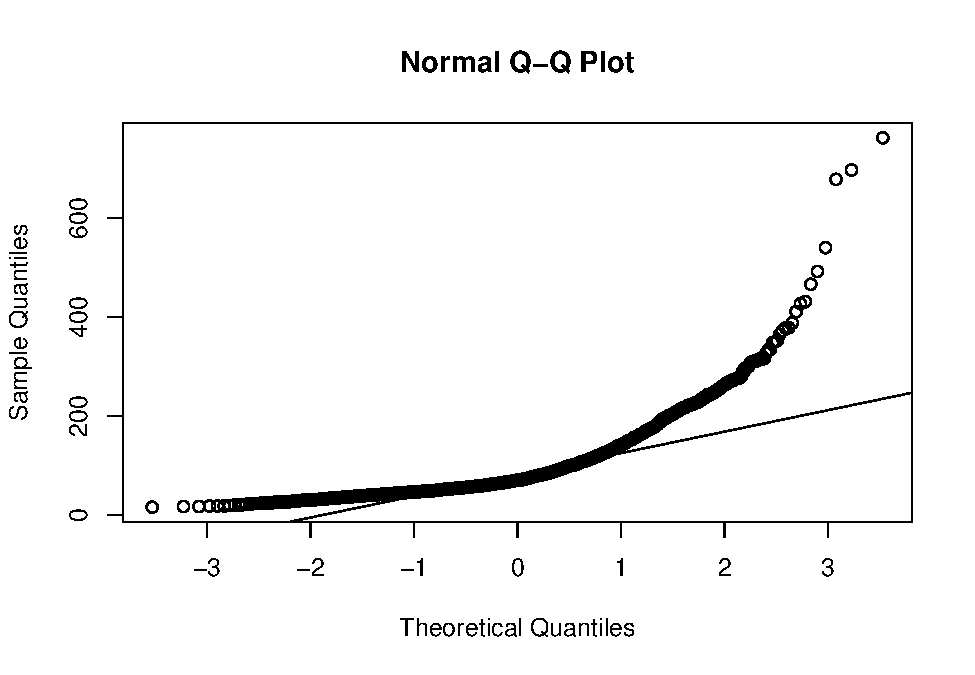
\includegraphics{Project_Code_files/figure-latex/question_2-1.pdf}

\begin{Shaded}
\begin{Highlighting}[]
\CommentTok{\# test for equal variance}
\FunctionTok{with}\NormalTok{(birds.subset, }\FunctionTok{bartlett.test}\NormalTok{(M\_tail }\SpecialCharTok{\textasciitilde{}}\NormalTok{ Display))}
\end{Highlighting}
\end{Shaded}

\begin{verbatim}
## 
##  Bartlett test of homogeneity of variances
## 
## data:  M_tail by Display
## Bartlett's K-squared = 71.043, df = 4, p-value = 0.00000000000001367
\end{verbatim}

\begin{Shaded}
\begin{Highlighting}[]
\FunctionTok{with}\NormalTok{(birds.subset, }\FunctionTok{bartlett.test}\NormalTok{(M\_tail }\SpecialCharTok{\textasciitilde{}}\NormalTok{ Mating\_System))}
\end{Highlighting}
\end{Shaded}

\begin{verbatim}
## 
##  Bartlett test of homogeneity of variances
## 
## data:  M_tail by Mating_System
## Bartlett's K-squared = 102.13, df = 4, p-value < 2.2e-16
\end{verbatim}

\begin{Shaded}
\begin{Highlighting}[]
\CommentTok{\# All significant; the variances are not equal}

\NormalTok{mating.anova }\OtherTok{\textless{}{-}} \FunctionTok{aov}\NormalTok{(}\AttributeTok{data =}\NormalTok{ birds.subset, M\_tail }\SpecialCharTok{\textasciitilde{}}\NormalTok{ Mating\_System }\SpecialCharTok{*}\NormalTok{ Display }\SpecialCharTok{*}\NormalTok{ Resource)}
\FunctionTok{summary}\NormalTok{(mating.anova)}
\end{Highlighting}
\end{Shaded}

\begin{verbatim}
##                                 Df  Sum Sq Mean Sq F value            Pr(>F)
## Mating_System                    4   59317   14829   3.548           0.00737
## Display                          4  164931   41233   9.865 0.000000129331941
## Resource                         2   18622    9311   2.228           0.10914
## Mating_System:Display           11  377637   34331   8.214 0.000000000000544
## Mating_System:Resource           3   13812    4604   1.102           0.34832
## Display:Resource                 8   35663    4458   1.067           0.38570
## Mating_System:Display:Resource   4   12473    3118   0.746           0.56109
## Residuals                      393 1642577    4180                          
##                                   
## Mating_System                  ** 
## Display                        ***
## Resource                          
## Mating_System:Display          ***
## Mating_System:Resource            
## Display:Resource                  
## Mating_System:Display:Resource    
## Residuals                         
## ---
## Signif. codes:  0 '***' 0.001 '**' 0.01 '*' 0.05 '.' 0.1 ' ' 1
## 3339 observations deleted due to missingness
\end{verbatim}

\begin{Shaded}
\begin{Highlighting}[]
\CommentTok{\# Reduce the model to achieve significance}
\CommentTok{\# Remove 3{-}way interaction}
\NormalTok{mating.anova}\FloatTok{.1} \OtherTok{\textless{}{-}} \FunctionTok{update}\NormalTok{(mating.anova, .}\SpecialCharTok{\textasciitilde{}}\NormalTok{.}\SpecialCharTok{{-}}\NormalTok{Mating\_System}\SpecialCharTok{:}\NormalTok{Display}\SpecialCharTok{:}\NormalTok{Resource) }
\FunctionTok{summary}\NormalTok{(mating.anova}\FloatTok{.1}\NormalTok{)}
\end{Highlighting}
\end{Shaded}

\begin{verbatim}
##                         Df  Sum Sq Mean Sq F value            Pr(>F)    
## Mating_System            4   59317   14829   3.557           0.00725 ** 
## Display                  4  164931   41233   9.891 0.000000122810784 ***
## Resource                 2   18622    9311   2.233           0.10851    
## Mating_System:Display   11  377637   34331   8.235 0.000000000000484 ***
## Mating_System:Resource   3   13812    4604   1.104           0.34714    
## Display:Resource         8   35663    4458   1.069           0.38371    
## Residuals              397 1655050    4169                              
## ---
## Signif. codes:  0 '***' 0.001 '**' 0.01 '*' 0.05 '.' 0.1 ' ' 1
## 3339 observations deleted due to missingness
\end{verbatim}

\begin{Shaded}
\begin{Highlighting}[]
\CommentTok{\# Remove Display:Resource}
\NormalTok{mating.anova}\FloatTok{.2} \OtherTok{\textless{}{-}} \FunctionTok{update}\NormalTok{(mating.anova}\FloatTok{.1}\NormalTok{, .}\SpecialCharTok{\textasciitilde{}}\NormalTok{.}\SpecialCharTok{{-}}\NormalTok{Display}\SpecialCharTok{:}\NormalTok{Resource) }
\FunctionTok{summary}\NormalTok{(mating.anova}\FloatTok{.2}\NormalTok{)}
\end{Highlighting}
\end{Shaded}

\begin{verbatim}
##                         Df  Sum Sq Mean Sq F value            Pr(>F)    
## Mating_System            4   59317   14829   3.552            0.0073 ** 
## Display                  4  164931   41233   9.877 0.000000123796776 ***
## Resource                 2   18622    9311   2.230            0.1088    
## Mating_System:Display   11  377637   34331   8.224 0.000000000000476 ***
## Mating_System:Resource   3   13812    4604   1.103            0.3477    
## Residuals              405 1690713    4175                              
## ---
## Signif. codes:  0 '***' 0.001 '**' 0.01 '*' 0.05 '.' 0.1 ' ' 1
## 3339 observations deleted due to missingness
\end{verbatim}

\begin{Shaded}
\begin{Highlighting}[]
\CommentTok{\# Remove Mating\_System:Resource}
\NormalTok{mating.anova}\FloatTok{.3} \OtherTok{\textless{}{-}} \FunctionTok{update}\NormalTok{(mating.anova}\FloatTok{.2}\NormalTok{, .}\SpecialCharTok{\textasciitilde{}}\NormalTok{.}\SpecialCharTok{{-}}\NormalTok{Mating\_System}\SpecialCharTok{:}\NormalTok{Resource) }
\FunctionTok{summary}\NormalTok{(mating.anova}\FloatTok{.3}\NormalTok{)}
\end{Highlighting}
\end{Shaded}

\begin{verbatim}
##                        Df  Sum Sq Mean Sq F value            Pr(>F)    
## Mating_System           4   59317   14829   3.550           0.00732 ** 
## Display                 4  164931   41233   9.870 0.000000124706921 ***
## Resource                2   18622    9311   2.229           0.10898    
## Mating_System:Display  11  377637   34331   8.217 0.000000000000477 ***
## Residuals             408 1704525    4178                              
## ---
## Signif. codes:  0 '***' 0.001 '**' 0.01 '*' 0.05 '.' 0.1 ' ' 1
## 3339 observations deleted due to missingness
\end{verbatim}

\begin{Shaded}
\begin{Highlighting}[]
\CommentTok{\# Remove Resource}
\NormalTok{mating.anova}\FloatTok{.4} \OtherTok{\textless{}{-}} \FunctionTok{update}\NormalTok{(mating.anova}\FloatTok{.3}\NormalTok{, .}\SpecialCharTok{\textasciitilde{}}\NormalTok{.}\SpecialCharTok{{-}}\NormalTok{Resource) }
\FunctionTok{summary}\NormalTok{(mating.anova}\FloatTok{.4}\NormalTok{)}
\end{Highlighting}
\end{Shaded}

\begin{verbatim}
##                        Df  Sum Sq Mean Sq F value     Pr(>F)    
## Mating_System           4  135625   33906   7.198 0.00001259 ***
## Display                 4  148286   37071   7.870 0.00000386 ***
## Mating_System:Display  12  229022   19085   4.052 0.00000526 ***
## Residuals             455 2143223    4710                       
## ---
## Signif. codes:  0 '***' 0.001 '**' 0.01 '*' 0.05 '.' 0.1 ' ' 1
## 3293 observations deleted due to missingness
\end{verbatim}

\begin{Shaded}
\begin{Highlighting}[]
\CommentTok{\# Everything is significant.}
\CommentTok{\# Not possible to run an AIC comparison because }
\CommentTok{\#the models do not contain the same number of observations.}
\CommentTok{\# Go with mating.anova.4, which is M\_tail \textasciitilde{} Mating\_System * Display}
\end{Highlighting}
\end{Shaded}

\begin{Shaded}
\begin{Highlighting}[]
\CommentTok{\#Grouping with Tukey HSD}
\NormalTok{anova.group }\OtherTok{\textless{}{-}} \FunctionTok{HSD.test}\NormalTok{(mating.anova}\FloatTok{.4}\NormalTok{, }\StringTok{"M\_tail"}\NormalTok{, }\AttributeTok{group =} \ConstantTok{TRUE}\NormalTok{)}
\NormalTok{anova.group}
\end{Highlighting}
\end{Shaded}

\begin{figure}
\centering
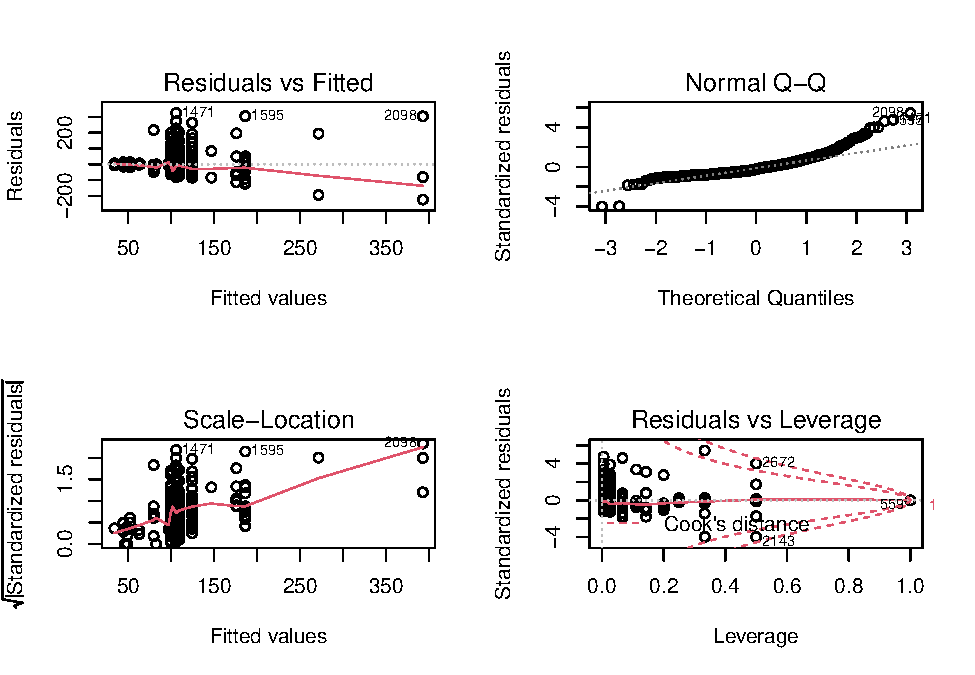
\includegraphics{Project_Code_files/figure-latex/q-2 residual-1.pdf}
\caption{Residual Plots for Question 2}
\end{figure}

\begin{figure}
\centering
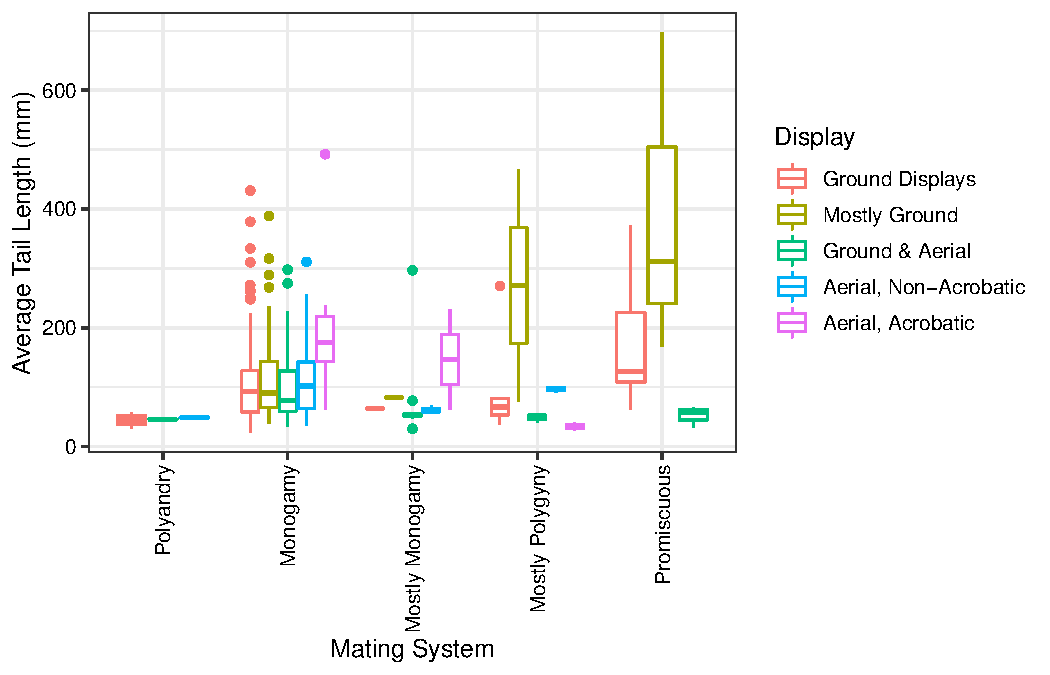
\includegraphics{Project_Code_files/figure-latex/q-2 plots-1.pdf}
\caption{Male Tail Length vs Mating Tactics}
\end{figure}

\newpage

\hypertarget{summary-and-conclusions}{%
\section{Summary and Conclusions}\label{summary-and-conclusions}}

\emph{Summarize your major findings from your analyses in a few
paragraphs. What conclusions do you draw from your findings? Relate your
findings back to the original research questions and rationale.}

\hypertarget{part-1}{%
\subsection{Part 1}\label{part-1}}

The interaction between female mass and tail size predicts clutch size
(p \textless{} 0.001, n = 1642, R\textsuperscript{2} = 0.022). The
effect of female tail size varies depending on the mass of the species.
* tail is negative; mass is positive; interaction is negative. I can't
remember how to interpret all this with the interaction

Limitations, Part 1 (do we need to run more assumption tests for this
one?) * R2 is low - model doesn't explain very much of the variance *
residuals plots - ?

\hypertarget{part-2}{%
\subsection{Part 2}\label{part-2}}

Mating system and display system together predict tail length (n = 476,
is the p-value just the interaction p-value for this one?)

Limitations, Part 2 * tail is not normally distributed (consider
transforming) * groups do not have equal variance (especially not
surprising with Mating System because the vast majority of the bird
species are Type 2 - Monogamous). * Need to check R2 for this one *
residual plots - ?

\newpage

\hypertarget{references}{%
\section{References}\label{references}}

Evans, M.R. 1999. The consequences of flight for the evolution of tail
ornaments in birds. In: Adams, N.J. \& Slotow, R.H. (eds) Proc. 22 Int.
Ornithol. Congr., Durban: 1823-1843. Johannesburg: BirdLife South
Africa.

Lislevand, T., Figuerola, J., and Székely, T. 2007. Avian body sizes in
relation to fecundity, mating system, display behavior, and resource
sharing. Ecology 88:1605.

\end{document}
